%!TEX root = main.tex
\definecolor{mygreen}{cmyk}{0.5,0,0.5,0.5}
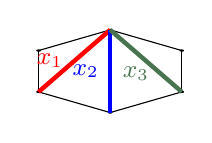
\begin{tikzpicture}[xscale = .6, yscale=0.3]
\tikzstyle{every node} = [font = \small]
\foreach \x in {0}
{
    \foreach \y in {-8}
    {
			\fill (\x,\y+1.75) circle (.05);
			%\fill (\x,\y+1.75) node [above] {\tiny{$1$}};
			\fill(\x+1.5158,\y+.875) circle (.05);
			%\fill (\x+1.5158,\y+.875) node [right] {\tiny{$2 $}};
			\fill (\x+1.5158,\y-.875) circle (.05);
			%\fill (\x+1.5158,\y-.875) node [right] {\tiny{$3$}};
			\fill(\x,\y-1.75) circle (.05);
			%\fill (\x,\y-1.75) node [below] {\tiny{$4$}};
			\fill(\x-1.5158,\y-.875) circle (.05);
			%\fill (\x-1.5158,\y-.875) node [left] {\tiny{$5$}};
			\fill (\x-1.5158,\y+.875) circle (.05);
			%\fill (\x-1.5158,\y+.875) node [left] {\tiny{$6$}};
		
			\draw [] (\x,\y+1.75)--(\x+1.5158,\y+.875); %v1 to v2
			\draw [] (\x+1.5158,\y+.875) -- (\x+1.5158,\y-.875); %v3 to v2
			\draw [] (\x+1.5158,\y-.875)--(\x,\y-1.75); %v4 to v3
			\draw [] (\x,\y-1.75) -- (\x-1.5158,\y-.875); %v5 to v4
			\draw [] (\x-1.5158,\y-.875)--(\x-1.5158,\y+.875); %v6 to v5
			\draw [] (\x-1.5158,\y+.875) -- (\x,\y+1.75); %v1 to v6
		
\draw [red, ultra thick] (\x,\y+1.75) -- (\x-1.5158,\y-.875) node[pos=0.5, left] {$x_1$};
\draw [blue, ultra thick] (\x,\y+1.75) -- (\x,\y-1.75) node[pos=0.5, left] {$x_2$};
\draw [mygreen, ultra thick] (\x,\y+1.75) -- (\x+1.5158,\y-.875) node[pos=0.7, left] {$x_3$};
	}
}
\end{tikzpicture}